\documentclass[12pt]{article}
% controlling the geometry of the page:
\usepackage[margin=1in, paperwidth=8.5in, paperheight=11in]{geometry} 
\usepackage{amsmath, amssymb} % useful math symbols and environments

\usepackage{multicol} % multiple columns side-by-side

\usepackage{amsthm} % Theorem-like environments
\theoremstyle{definition} % Without this line, theorem statements (and therefore problem statements etc.) show up in italic text.
\newtheorem{conjecture}{Conjecture}
\newtheorem{problem}{Problem}

% pretty colors!
\usepackage[dvipsnames]{xcolor}
\colorlet{darkgrey}{black!70}
\colorlet{darkgreen}{green!50!black}

\usepackage{tikz} % for drawing diagrams
\usetikzlibrary{arrows,automata,positioning} 
\usetikzlibrary{decorations.markings}
\usetikzlibrary{decorations.pathreplacing}
\usetikzlibrary{patterns}
\usetikzlibrary{shapes.geometric}

%%---------------------------------------------------------------------------
%% included from visualalgebra.sty (see the beamer folder)
%% TEXT COLORS
%%
\definecolor{xRed}{rgb}{.9,0,0}       
\definecolor{xBlue}{rgb}{0,0,.9}      
\definecolor{xGreen}{HTML}{009000}   %% "Islamic green"
\definecolor{xPurple}{HTML}{D14FFF}  
\definecolor{xOrange}{HTML}{F56600}  %% "Clemson orange"

\newcommand{\Alert}[1]{\textcolor{xRed}{#1}}
\newcommand{\Balert}[1]{\textcolor{xBlue}{#1}}
\newcommand{\Galert}[1]{\textcolor{xGreen}{#1}}
\newcommand{\Palert}[1]{\textcolor{xPurple}{#1}}
\newcommand{\Oalert}[1]{\textcolor{xOrange}{#1}}
\newcommand{\Walert}[1]{\textcolor{white}{#1}}

%% vertices in cayley graphs
\tikzset{v/.style={circle, draw, fill=lightgray,inner sep=0pt, 
  minimum size=6mm}}

%% Edge colors
%%
\definecolor{eRed}{rgb}{1,0,0}      % Cayley diagram edges
\definecolor{eBlue}{rgb}{0,0,1}     % Cayley diagram edges
\definecolor{eGreen}{HTML}{7EC636}  % Goodnotes green (a little darker)
\definecolor{eGreen}{HTML}{3CAC13}  % I like this a litte better
\definecolor{ePurple}{HTML}{D287FF} % Close to goodnotes 
\colorlet{eOrange}{orange}

%% Edge styles 
%%
\tikzset{r/.style={draw, very thick, eRed, -stealth}}  % Red -->
\tikzset{rr/.style={draw, very thick, eRed}}           % Red ---
\tikzset{b/.style={draw, very thick, eBlue, -stealth}} % Blue -->
\tikzset{bb/.style={draw, very thick, eBlue}}          % Blue ---
\tikzset{g/.style={draw, very thick, eGreen, -stealth}} % Green -->
\tikzset{gg/.style={draw, very thick, eGreen}}          % Green ---
%%---------------------------------------------------------------------------

\usepackage{graphicx} % for inserting figures with \includegraphics
\usepackage{setspace} % for controlling space between lines, paragraphs, etc.

\usepackage{fancyhdr} % for controlling headers and footers
\usepackage{newtx} % changes the default font family
\usepackage[shortlabels]{enumitem} % controllable labels for ordered and unordered lists

\usepackage{hyperref} % controls hyperlinks, both internal and external
\hypersetup{
    colorlinks=true,
    urlcolor=blue,
}

\setlength{\headheight}{14.5pt}
\newcommand{\Q}{\mathbb{Q}}
\newcommand{\R}{\mathbb{R}}
\newcommand{\Z}{\mathbb{Z}}
\newcommand\inv{^{-1}} % I am very tired of typing ^{-1}
\def\<{\langle}
\def\>{\rangle}
\DeclareMathOperator\Rect{\mathbf{Rect}}
\DeclareMathOperator\Tri{\mathbf{Tri}}
\DeclareMathOperator\Sq{\mathbf{Sq}}
\DeclareMathOperator\Light{\mathbf{Light}}
\DeclareMathOperator{\lcm}{lcm}

\newenvironment{red}{\color{red}}{\ignorespacesafterend}

% I don't like how LaTeX renders section headings by default
\renewcommand{\section}[1]{\begin{center} \textbf{#1} \\\end{center}}
%
\setlength{\parindent}{0in}
%\oddsidemargin=-.25in
\allowdisplaybreaks
\pagestyle{fancy}
\renewcommand{\headrulewidth}{0pt}
\lhead{MATH 312}
\rhead{Spring 2025}
%\lfoot{\copyright\ CLEAR Calculus 2010}
\cfoot{}
\renewcommand{\thefootnote}{*} 
\hyphenpenalty=10000 % LaTeX by default really likes hyphenating things

% all the stuff above this line is called the preamble...
%##################################################################
\begin{document} % this is always the first line of what's actually produced
\section{Homework \#3} % notice that if you want the character # to appear, you have to "escape" it with a backslash

HW due Sunday 2/9 by pdf upload to Canvas; .tex source on the \href{https://github.com/rhinopotamus/math312}{MATH 312 github repo}.

\subsection*{Stuff about permutation groups and $S_n$}

\begin{problem}
    There are three canonical types of generating sets for $S_n$:
    \begin{itemize}
        \item A \Galert{transposition} and an \Alert{$n$-cycle},
        e.g.,: 
        \(
        S_n=\<\,\Galert{(1\;2)},\;\;\Alert{(1\;2\,\cdots\,
            n\!-\!1\;\;n)}\>\,.
        \)
%------------ LaTeX note: Note the use of "\;" to force there to be a bit more space between the elements in cycle notation. There are lots of similar space-in-math-mode commands, such as "\ ", "\,", "\.", and "\:".
% https://www.overleaf.com/learn/latex/Spacing_in_math_mode
        
        \item \Balert{Adjacent transpositions}:
        \(
        S_n=\<\,(1\;2),\;(2\; 3),\;\dots,\; (n-1\;\;n)\>\,. 
        \)

        \item \Palert{Overlapping transpositions}, e.g.,:
        \(
        S_n=\<\,(1\;2),\;(1\; 3),\;\dots,\; (1\;\;n)\>\,. 
        \)
    \end{itemize}
    ``It should be intuitive'' that any one of these types of generating sets works to get you the full $S_n$. Write some human words (not a proof) explaining why. It may be helpful to play around with a row of $n$ objects or a small deck of cards.
\end{problem}

\begin{problem}
    Suppose that $g, h \in G$. We mentioned in class that the \textit{conjugate} of $h$ by $g$ is the element $ghg\inv$. The \textit{conjugacy class} of $h$ is the set of all the possible conjugates of $h$: $\{ghg\inv \mid g\in G\}.$
    \begin{itemize}
        \item Find the conjugacy classes of all six elements of $S_3$. (If you use the permutation calculator, make sure you're multiplying left-to-right!) 
        \item If you are having fun, find the conjugacy classes of all 24 elements of $S_4$.
        \item Meditate upon the following wisdom: Conjugation in $S_n$ is essentially ``relabeling'' the numbers in the original permutation.
    \end{itemize}
\end{problem}

\begin{problem}
    Suppose $\sigma \in S_n$, and that $|\sigma| = k$. 
    \begin{itemize}
        \item Explain why $\sigma^k$ is an even permutation.
        \item Suppose that $\sigma$ is an odd permutation. Is $k$ even or odd? How do you know?
        \item Conclude that a cycle of odd length is an even permutation. Feel moderate annoyance.
    \end{itemize}
\end{problem}

\begin{problem}
    Play a bit more with Cayley's theorem:
    \begin{itemize}
        \item Extract from the Cayley diagram of $C_4\times C_2 = \< \Alert{r}, \Balert{b} \>$ the two permutations that describe its arrows, and therefore describe $C_4 \times C_2$ as a subgroup of a symmetric group.
        \item Do the same for $Q_8 = \< \Alert{i}, \Balert{j}, \Galert{-1} \>$.

        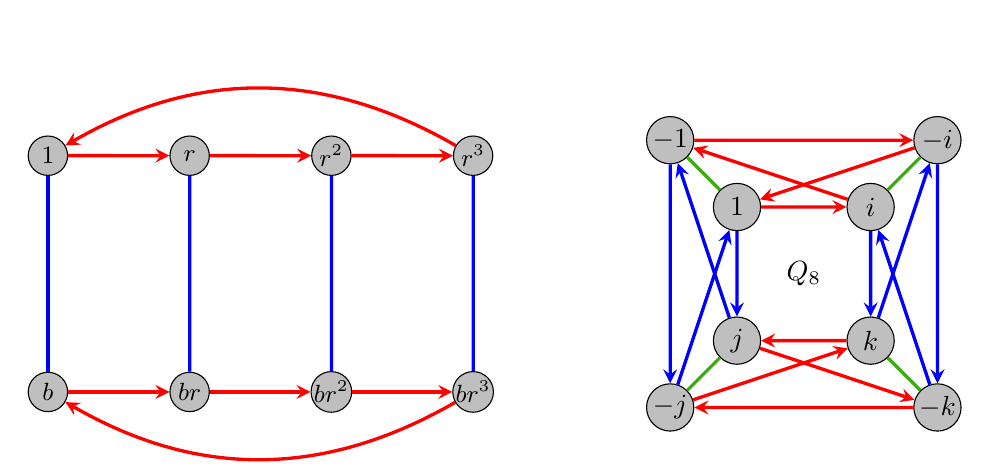
\begin{tikzpicture}[scale = 1.2]
            \begin{scope}[shift = {(-4, 0)}]
                \tikzstyle{v} = [circle, draw, fill=lightgray,inner sep=0pt, 
                    minimum size=5mm]  
                \tikzstyle{every node}=[font=\small]
                %%
                \node (10) at (0,2.5) [v] {$1$};
                \node (11) at (1.5,2.5) [v] {$r$};
                \node (12) at (3,2.5) [v] {$r^2$};
                \node (13) at (4.5,2.5) [v] {$r^3$};
                \node (00) at (0,0) [v] {$b$};
                \node (01) at (1.5,0) [v] {$br$};
                \node (02) at (3,0) [v] {$br^2$};
                \node (03) at (4.5,0) [v] {$br^3$};
                \draw [r] (00) to (01); 
                \draw [r] (01) to (02);
                \draw [r] (02) to (03);
                \draw [r] (03) to [bend left] (00);
                \draw [r] (10) to (11); 
                \draw [r] (11) to (12);
                \draw [r] (12) to (13);
                \draw [r] (13) to [bend right] (10);
                \draw [bb] (00) to (10);
                \draw [bb] (01) to (11);
                \draw [bb] (02) to (12);
                \draw [bb] (03) to (13);
            \end{scope}
            \begin{scope}[shift = {(4, 1.25)}]
                \node (1) at (135:1) [v] {$1$};
                \node (i) at (45:1) [v] {$i$};
                \node (k) at (-45:1) [v] {$k$};
                \node (j) at (-135:1) [v] {$j$};
                \node (-1) at (135:2) [v] {$-1$};
                \node (-i) at (45:2) [v] {$-i$};
                \node (-k) at (-45:2) [v] {$-k$};
                \node (-j) at (-135:2) [v] {$-j$};
                \node at (0,0) {\normalsize $Q_8$};
                %%
                \path[r] (1) to (i);
                \path[r] (i) to (-1);
                \path[r] (-1) to (-i);
                \path[r] (-i) to (1);
                %%
                \path[r] (k) to (j);
                \path[r] (j) to (-k);
                \path[r] (-k) to (-j);
                \path[r] (-j) to (k);
                %%
                \path[b] (i) to (k);
                \path[b] (k) to (-i);
                \path[b] (-i) to (-k);
                \path[b] (-k) to (i);
                %%
                \path[b] (1) to (j);
                \path[b] (j) to (-1);
                \path[b] (-1) to (-j);
                \path[b] (-j) to (1);
                %%
                \path[gg] (1) to (-1);
                \path[gg] (j) to (-j);
                \path[gg] (i) to (-i);
                \path[gg] (k) to (-k);
            \end{scope}
          \end{tikzpicture}
    \end{itemize}
    
\end{problem}

\subsection*{Stuff about direct products}

\begin{problem}
    I want to make the relationship between the inflate-the-Cayley-diagram description and the ordered-pairs description of a direct product a bit more evident. Say that $\Alert{C_4} = \<\Alert{r} \mid \Alert{r}^4 = 1\>$ and $\Balert{C_3} = \< \Balert{b} \mid \Balert{b}^3 = 1\>$. 
    \begin{itemize}
        \item Write out all 12 elements of $\Alert{C_4}\times \Balert{C_3}$ as ordered pairs. (They will all look like $(\Alert{r}^k, \Balert{b}^j)$.)
        \item Use the inflation procedure to draw the Cayley diagram of $\Alert{C_4}\times \Balert{C_3}$.
        \item Label each node in your Cayley diagram with the corresponding ordered pair.
        \item (Bonus problem: Is $\Alert{C_4}\times \Balert{C_3}$ ``secretly cyclic''?)
    \end{itemize}
\end{problem}

\begin{problem}
    Explore $\Alert{C_2} \times \Balert{C_2} \times \Galert{C_2}$.
    \begin{itemize}
        \item Figure out how to repeat the inflation process to draw a Cayley diagram.
        \item Compute the orbits of each of the 8 elements and draw a cycle graph.
        \item Is this a new group? Groups of order 8 we already know are $C_8$, $C_4 \times C_2$, $D_4$, and $Q_8$. 
    \end{itemize}
\end{problem}

\begin{problem}
    Prove using algebra that $A\times B$ is abelian \Alert{if and only if} both $A$ and $B$ are abelian.

    \textit{Hint:} Remember that an \Alert{``if and only if''} statement is actually looking for \textit{two} proofs. I will provide you with the proof frames for each one:
    \begin{multicols}{2}
        ($\Rightarrow$) Suppose that $A$ and $B$ are both abelian.

        \ldots

        Therefore, $A\times B$ is abelian.

        ($\Leftarrow$) Suppose that $A\times B$ is abelian.

        \ldots

        Therefore, $A$ and $B$ are both abelian.
    \end{multicols}

    Remember that filling in the second line and the second-to-last line, usually by unpacking a definition (here: what does ``abelian'' mean again?), is a good way to proceed after writing the proof frame.
    
\end{problem}

\begin{problem}
    Here we'll explore when the product of cyclic groups is ``secretly cyclic''.
    \begin{enumerate}[(a)]
        \item Say you have a generic group $G$ such that $|G| = n$. Suppose further that you found an element $g\in G$ such that $|g| = n$. Prove that $G$ is cyclic. (Hint: look at the orbit of $g$, and think about the definition of $|g|$.)

        \item Suppose that $a, b \in \Z$ are relatively prime. (Google it if you don't remember what this means.) Fact: $\lcm(a, b) = ab.$ Optional challenge: prove it.

        \item Consider the direct product $\Z_a \times \Z_b$, with $a$ and $b$ relatively prime. What is $|(1,1)|$?

        (\textbf{\Alert{NOTE TYPO FIX:}} I had previously written $C_a \times C_b$, in which the element $(1,1)$ would represent the identity. I could also have said, suppose that $C_a = \<g\>$ and $C_b = \<h\>$ and then think about the element $(g, h)\in C_a \times C_b$, but I think it's cleaner this way.)

        \item Conclude that $\Z_a \times \Z_b \cong \Z_{ab}.$
    \end{enumerate}
\end{problem}

\end{document}

